\documentclass[bibnumbers, palatino]{apuntes}

\title{Ecuaciones en Derivadas Parciales}
\author{Elena Gutiérrez Viedma}
\date{15/16 C2}

% Paquetes adicionales
\usepackage{tikztools}
\usepackage{fancysprefs}
\usepackage{enumitem}
\usepackage{fastbuild}
\usepackage{titlesec}
\usepackage{xfrac}
\usepackage{graphicx}
\graphicspath{{img/}}
% --------------------





\titleclass{\subsubsubsection}{straight}[\subsection]

\newcounter{subsubsubsection}[subsubsection]
\renewcommand\thesubsubsubsection{}
\renewcommand\theparagraph{\thesubsubsubsection.\arabic{paragraph}} % optional; useful if paragraphs are to be numbered

\titleformat{\subsubsubsection}
  {\normalfont\normalsize\bfseries}{\thesubsubsubsection}{1em}{}
\titlespacing*{\subsubsubsection}
{0pt}{3.25ex plus 1ex minus .2ex}{1.5ex plus .2ex}

\makeatletter
\renewcommand\paragraph{\@startsection{paragraph}{5}{\z@}%
  {3.25ex \@plus1ex \@minus.2ex}%
  {-1em}%
  {\normalfont\normalsize\bfseries}}
\renewcommand\subparagraph{\@startsection{subparagraph}{6}{\parindent}%
  {3.25ex \@plus1ex \@minus .2ex}%
  {-1em}%
  {\normalfont\normalsize\bfseries}}
\def\toclevel@subsubsubsection{4}
\def\toclevel@paragraph{5}
\def\toclevel@paragraph{6}
\def\l@subsubsubsection{\@dottedtocline{4}{7em}{4em}}
\def\l@paragraph{\@dottedtocline{5}{10em}{5em}}
\def\l@subparagraph{\@dottedtocline{6}{14em}{6em}}

\precompileTikz

\setcounter{secnumdepth}{4}
\setcounter{tocdepth}{4}

\bibliographystyle{plainnat}

\begin{document}
\pagestyle{plain}

% http://tex.stackexchange.com/a/14243
%\relpenalty=10000
%\binoppenalty=10000
\section{Parcial 2 de E.D.P.}

\begin{problem} Tenemos la siguiente ecuación de onda. \[ \begin{cases}
u_{tt} - u_{xx} = 0	& x \in (0,4),\; t > 0 \\
u(0,t) = 0 = u(4,t) & t > 0 \\
u(x,0) = f(x)\\
u_t(x,0) = 0 	
\end{cases} \]
donde $f(x)$ tiene la siguiente expresión:
\[ f(x) = \begin{cases}
-(x-3)(x-1)	& x \in [1,3]\\
0 & x \in (0,1)\cup(3,4)\\
\end{cases} \]
Se pide:
\begin{enumerate}
\item Hallar el máximo y mínimo de la solución $u(x,t)$ en el instante $t=1$ (valores máximo y mínimo, y puntos en los que se alcanza).
\item Hallar el máximo y mínimo de la solución $u(x,t)$ en el instante $t=2$ (valores máximo y mínimo, y puntos en los que se alcanza).
\item Calcular la energía de la solución $u(x,t)$ en el instante $t$.
\end{enumerate}
\solution
\textbf{Apartado 1.} \newline

Sabemos que $u(0,t)=u(4,t)=0~\forall t>0$, de modo que $u(0,1)=u(4,1)=0$. Si a esto le añadimos el comportamiento de $u(x,t)$ en el resto del intervalo $[0,4]$ tenemos:
\[ u(x,1) = \begin{cases}
0	& x=0\\
\frac{1}{2}\{f(x+1)+0\}=-\frac{1}{2}x(x-2)	& x \in (0,2)\\
[\frac{1}{2}\{f(x+1)+f(x-1)\}]_{x=2}=\frac{1}{2}\{f(3)+f(1)\}=0	& x=2\\
\frac{1}{2}\{0+f(x-1)\}=-\frac{1}{2}(x-4)(x-2)	& x \in (2,4)\\
0	& x=4\\
\end{cases} \]
Buscamos el máximo y el mínimo de $u(x,1)$. Llamamos $g(x) = -\frac{1}{2}x(x-2) $, con $x\in (0,2)$ y $h(x)=-\frac{1}{2}(x-4)(x-2)$, con $x\in (2,4)$
\begin{itemize}
\item $g'(x) = 1-x = 0 \implies x_0 = 1$.\\ Además, $g''(1) \leq 0 \implies$ $x_0 = 1$ es un máximo en $(0,2)$, con $g(1)=\frac{1}{2}$.
\item $h'(x) = 3-x = 0 \implies x_1 = 3$.\\ Además, $h''(3) \leq 0 \implies$ $x_1 = 3$ es un máximo en $(2,4)$, con $h(3)=\frac{1}{2}$.
\end{itemize}

Esta información es la que recoge el gráfico de la Figura \ref{fig:onda}.
\begin{figure}[hbtp]
\centering
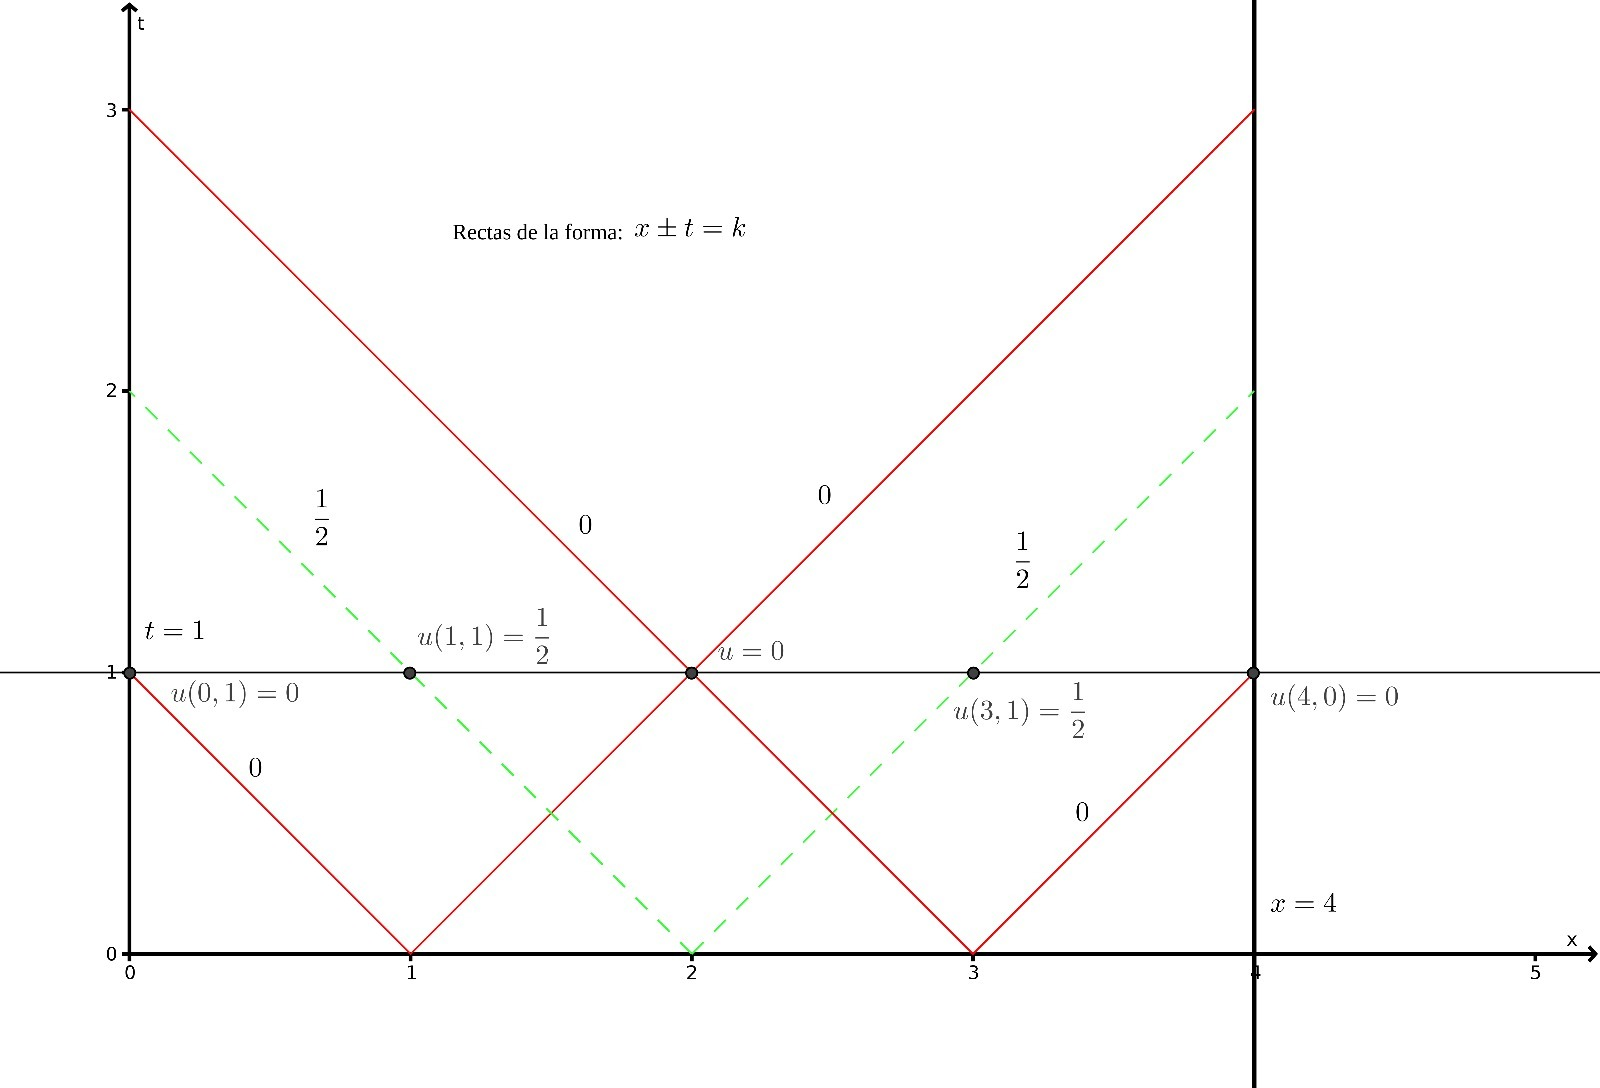
\includegraphics[width =1.1\textwidth]{img1}
\caption{Solución $u(x,t)$ para la ecuación de onda en $t=1$}
\label{fig:onda}
\end{figure}

Es decir, la onda inicial ($t=0$), cuya expresión venía dada por $f$, en el instante $t=1$ se encuentra dividida en 2 ondas cada una de ellas viajando a velocidad 1 hacia la derecha e izquierda respectivamente y con una amplitud igual a la mitad de la amplitud incial.

\newpage Con esto podemos contestar a la pregunta formulada:
\begin{itemize}
\item \textbf{Máximo de $u(x,1)$}: $u=\frac{1}{2}$. Se alcanza en $x=1$ y $x=3$.
\item \textbf{Mínimo de $u(x,1)$}: $u=0$. Se alcanza en $x=0$, $x=2$ y $x=4$.
\end{itemize}
\newpage
\textbf{Apartado 2.} \newline

En este caso, la Figura \ref{fig:onda2} muestra $u(x,t)$ cuando $t=2$.
\begin{figure}[hbtp]
\centering
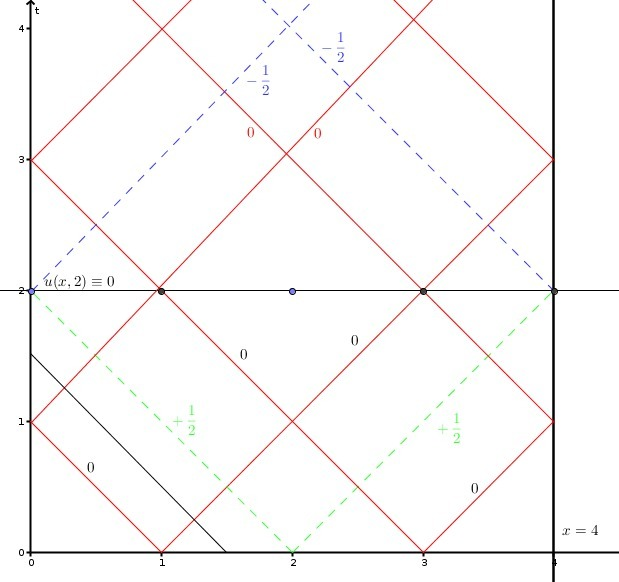
\includegraphics[width =0.9\textwidth]{img2}
\caption{Solución $u(x,t)$ para la ecuación de onda en $t=2$}
\label{fig:onda2}
\end{figure}

En este caso se observa lo siguiente:
\begin{itemize}
\item $u(x,2) = 0$ si $x\in [1,3]$ . Las dos ondas que viajaban a velocidad 1 hacia la izquierda y la derecha desde $x=2$ en $t=1$, en $t=2$ ya han recorrido una unidad de distancia en cada dirección, quedando el intervalo [1,3] con amplitud 0 ($u=0$).
\item $u(x,2) = 0$ si $x\in [0,1)\cup(3,4]$. En $t=2$, la mitad de cada onda que viajaba en cada dirección ha topado con los extremos en $x=0$ y $x=4$, y se ha reflejado. El efecto de la reflexión contrarresta a la otra mitad de la onda que todavía no ha llegado a la pared, anulando su amplitud ($u=0$).

De modo que tenemos:
\begin{itemize}

\item \textbf{Máximo de $u(x,2)$}: $u=0$. Se alcanza en todo el intervalo $[0,4]$.
\item \textbf{Mínimo de $u(x,2)$}: $u=0$. Se alcanza en todo el intervalo $[0,4]$.
\end{itemize}
\newpage
\textbf{Apartado 3.}\newline

Sabemos que la energía del sistema viene dada por la siguiente expresión:
$$E(t)=\frac{1}{2}\int^{4}_{0}(u_{x}^2 + u_{t}^2 )dx$$
Además sabemos:
\begin{itemize}
\item $E(t) = $cte. $~\forall t > 0 \implies E(0) =$ cte.
\item $u(x,0) = f(x),~ \forall x\in (0,4)$
\item $u_t(x,0) = 0,~\forall x \in(0,4)$
\end{itemize}
Entonces:
$$\frac{1}{2}\int^{4}_{0}(f'(x))^2dx = \frac{1}{2}\int^{3}_{1}(-2x+4)^2dx = \frac{1}{2}\int^{3}_{1}(4x^2 - 16x +16)dx =  \frac{4}{3}$$
\end{itemize}
\end{problem}

\newpage
\begin{problem}
Consideramos la ecuación del calor:
\[u_t -u_{xx} = 0, x\in(0,\pi), t>0,\]
con condiciones de contorno
\[u(0,t) = u (\pi,t) = 0,\]
y con dato inicial
\[u(x,0) = f(x) = x.\]

\begin{itemize}
\item Aplicar el método de separación de variables, y encontrar la serie de Fourier asociada a la solución del problema (escribir al menos los cinco primeros términos no nulos de la serie).
\item Demostrar que, para $t>0$, la serie converge (en el sentido apropiado) a una función $u(x,t)$, que es derivable hasta cualquier orden, y es solución clásica de la ecuación.
\item Discutir la convergencia (uniforme, puntual o en $L^2([0,\pi])$) de la serie en el instante $t=0$.
\end{itemize}
\solution
\textbf{Apartado 1.}\newline
\end{problem}
Supongamos $u(x,t) = X(x)T(t)$. Entonces, \[\begin{cases}u_{t} = X(x)T'(t)\\u_{xx} = T(t)X''(x)\end{cases}\] y nuestra ecuación queda: \[X(x)T'(t) = T(t)X''(x) \Leftrightarrow \frac{T'(t)}{T(t)} = \frac{X''(x)}{X(x)} = \lambda,~\lambda \in \mathbb{R}\]
\begin{enumerate}
\item Resolvemos la E.D.O en $X(x)$:~$X''(x) = \lambda X(x)$
\begin{enumerate}
\item $\lambda = 0$: $X''(x) = 0 \implies$ \[ \begin{cases}X(x) = a + bx\\ X(0) = 0 \Leftrightarrow a = 0\\X(\pi) = 0 \Leftrightarrow b\pi = 0 \Leftrightarrow b = 0 \end{cases}\]
Conclusión: Si $\lambda  = 0$, entonces $X(x)\equiv 0$ (solución trivial).
\item $\begin{cases}\lambda > 0\\ \lambda = \mu^2\end{cases}$: $X''(x) = \mu^2 X(x) \implies$ \[ \begin{cases}X(x) = Ae^{\mu x} + Be^{-\mu x}\\ X(0) = A + B \Leftrightarrow A = -B\\X(\pi) = Ae^{\mu \pi} - Ae^{-\mu \pi}  = 0 \Leftrightarrow A(e^{\mu \pi} - e^{-\mu \pi} ) = 0 \Leftrightarrow A  = 0 \end{cases}\]
Conclusión: Si $\lambda  > 0$, entonces $X(x)\equiv 0$ (solución trivial).
\item $\begin{cases}\lambda < 0\\ \lambda = -\mu^2\end{cases}$: $X''(x) = -\mu^2 X(x) \implies$ \[ \begin{cases}X(x) = Acos{\mu x} + Bsen{\mu x}\\ X(0) = A + 0 \Leftrightarrow A = 0\\X(\pi) = Bsen{\mu \pi}  = 0 \Leftrightarrow  \begin{cases}B = 0~(sol. trivial) \\ \mu\pi = k\pi \implies \mu = k \end{cases}\end{cases}\]
Conclusión: Si $\lambda  < 0$, entonces $X_k(x)\equiv B_ksen(kx),~$con $k\in \mathbb{N}$ y $\lambda_k = -k^2$.
\end{enumerate}

\item Resolvemos la E.D.O. en $T(t)$:~$T'(t) = \lambda_k T(t)\Leftrightarrow T'(t) = -k^2T(t) \implies \\T_k(t) = \alpha_ke^{-k^2t}$ 
\end{enumerate}
Llamando $A_k = B_k\alpha_k$, tenemos $u_k(x,t) = X_k(x)T_k(t) = B_ksen(kx)\alpha_ke^{-k^2t} = A_k sen(kx)e^{-k^2t} $.
Escribimos el candidato a solución en forma de serie:
\begin{equation}
u(x,t) = \sum^{\infty}_{k=1}A_ksen(kx)e^{-k^2t}
\label{eq}
\end{equation}

Usamos el dato inicial para determinar el valor de los coeficientes $A_k$:
\[u(x,0) = \sum^{\infty}_{k=1}A_ksen(kx) = x\]

Para poder determinar el valor de los $A_k$ debemos desarrollar la función $f(x) = x$ con $x\in[0,\pi]$ en serie de senos. Para ello, calculamos una extensión \emph{impar} de $f$ en el intervalo $[-\pi,\pi]$ a la que llamaremos $\hat{f}$ y que viene dada por:
\[\hat{f}(x) = \begin{cases}f(x) & x\in [0,\pi]\\-f(-x) & x\in [-\pi,0]\end{cases}\]

La razón por la que calculamos la extensión impar es que así los coeficientes $\{a_k\}_{k=1}^{\infty}$ que acompañan a los cosenos en el desarrollo,
\[\hat{f}(x) = \frac{a_0}{2} + \sum^{\infty}_{k=1} a_k cos(kx) + b_k sen(kx) \]

así como el coeficiente $a_0$, se anulan quedando su desarrollo de Fourier en senos, tal y como lo necesitamos. La razón por la que estos coeficientes se anulan es la siguiente:
\begin{enumerate}
\item $a_0  = \frac{1}{\pi}\int^{\pi}_{-\pi} \hat{f}(x)dx = 0$. (La integral de una función $\hat{f}$ impar en un intervalo simétrico es 0).
\item $a_k = \frac{1}{\pi}\int^{\pi}_{-\pi} \hat{f}(x)cos(kx)dx = 0$. (El producto de una función impar y una par es impar, y de nuevo por 1.).
\end{enumerate}
Por otra parte calculamos los $b_k$, que no van a ser 0:
\begin{enumerate}
\item $b_k = \frac{1}{\pi}\int^{\pi}_{-\pi}\hat{f}(x)sen(kx)dx = \frac{2}{\pi}\int^{\pi}_{0}f(x)sen(kx)dx  = \frac{2}{\pi}\int^{\pi}_{0}x sen(kx)dx =\left.\frac{2}{\pi}(-x\frac{coskx}{k} + \frac{1}{k^2}senkx)\right|^{\pi}_{0} = \frac{2(-1)^{k+1}}{k} $
\end{enumerate}

Luego:
\[f(x) = \sum^{\infty}_{k=1}\frac{2(-1)^{k+1}}{k} sen(kx), ~x\in[0,\pi]\]

Por tanto,
\[u(x,0) = \sum^{\infty}_{k=1}A_ksen(kx) = x = \sum^{\infty}_{k=1}\frac{2(-1)^{k+1}}{k} sen(kx),\]

así tenemos que los primeros 5 coeficientes no nulos $A_k$ de la serie (\ref{eq}) son:
\[A_1 = 2,~A_2 = -1,~A_3 = \frac{2}{3},~A_4 = -\frac{1}{2},~A_5 = \frac{2}{5}\]\newline
\textbf{Nota:} \newline De momento, no hemos demostrado nada sobre la convergencia de esta serie, de modo que el signo $=$ que utilizamos está "entre comillas".\newline
\\
\textbf{Apartado 2.}\newline

Con los resultados del apartado anterior tenemos que:
\begin{equation}
\label{eq3}
u(x,t) \sim  \sum^{\infty}_{k=1} \frac{2(-1)^{k+1}}{k} sen(kx)e^{-k^2t}, ~ t>0, ~ x\in(0,\pi)
\end{equation}

A continuación demostraremos que podemos poner el signo "$=$" en el sentido de la convergencia uniforme, y por consiguiente, en el sentido de la convergencia puntual. Para ello, usaremos el Criterio de Convergencia de Weierstrass. 

Sea $$\Phi_k(x,t) = \frac{2(-1)^{k+1}}{k} sen(kx)e^{-k^2t}. $$ basta demostrar que existe $M_k$ tal que \mbox{$|\Phi_k|\leq M_k$},~$\forall x\in[0,\pi]$ tal que $\sum^{\infty}_{k=1}M_k<\infty$. Aplicando el Criterio de Weierstrass tendríamos que $\sum^{\infty}_{k=1}\Phi_{k}(x,t) = u(x,t)$ converge uniformemente en $[0,\pi]$ con $t>0$.

Sabemos que:
$$|\Phi_k(x,t)| = |\frac{2(-1)^{k+1}}{k} sen(kx)e^{-k^2t}|\leq |\frac{2}{{k}e^{-k^2t}}| = M_k(t)$$

De modo que, si $t>0$ se verifica:

\[\sum_{k=1}^{\infty} |M_k(t)| = \sum_{k=1}^{\infty} |\frac{2}{{k}e^{-k^2t}}|<\infty\]

Por el criterio de Weierstrass concluimos que la serie $\sum^{\infty}_{k=1} \frac{2(-1)^{k+1}}{k} sen(kx)e^{-k^2t}$ converge uniformemente con $t>0, ~ x\in(0,\pi)$. Por tener convergencia uniforme, concluimos convergencia puntual también en $t>0, ~ x\in(0,\pi)$.

Por otra parte, según el siguiente teorema visto en clase:

\begin{theorem}
\label{teorema}
Sea $\{\psi_n\}_{n=1}^{\infty}$ una sucesión de funciones tal que verifica:
\[\begin{cases}\sum^{N}_{n=1}\psi_n\longrightarrow f ~unif. ~en ~(a,b)\\ \sum^{N}_{n=1}\psi'_n\longrightarrow g ~unif. ~en ~(a,b) \end{cases} \implies f~derivable~en~(a,b)~y~f'=g\]
\end{theorem}

Aplicamos el Teorema con $f = u$ y $g = u_t$:
$$u_t  \sim \sum^{\infty}_{k=1} \frac{2(-1)^{k+1}}{k} sen(kx)(-k^2)e^{-k^2t}, ~ t>0, ~ x\in(0,\pi)$$

Por el Criterio de Convergencia de Weierstrass  con $M_k(t) = \frac{2(-k)}{e^{k^2t}}$ tenemos que la serie converge uniformemente con $t>0$ en $(0,\pi)$, y aplicando el Teorema se concluye:

\begin{equation}
u_t  = \sum^{\infty}_{k=1} \frac{2(-1)^{k+1}}{k} sen(kx)(-k^2)e^{-k^2t}, ~ t>0, ~ x\in(0,\pi)
\label{eq2}
\end{equation}

De nuevo aplicamos el Teorema con $f = u$ y $g = u_x$:
$$u_x  \sim \sum^{\infty}_{k=1} \frac{2(-1)^{k+1}}{k} k cos(kx)e^{-k^2t}, ~ t>0, ~ x\in(0,\pi)$$

Por el Criterio de Convergencia de Weierstrass  con $M_k(t) = \frac{2}{e^{k^2t}}$ tenemos que la serie converge uniformemente con $t>0$ en $(0,\pi)$, y aplicando el Teorema se concluye:

$$u_x  = \sum^{\infty}_{k=1} \frac{2(-1)^{k+1}}{k} k cos(kx)e^{-k^2t}, ~ t>0, ~ x\in(0,\pi)$$


Por último, aplicamos el Teorema con $f = u_x$ y $g = u_{xx}$:
$$u_{xx}  \sim \sum^{\infty}_{k=1} \frac{2(-1)^{k+1}}{k} k^2 (-sen(kx))e^{-k^2t}, ~ t>0, ~ x\in(0,\pi)$$

Por el Criterio de Convergencia de Weierstrass  con $M_k(t) = \frac{2k}{e^{k^2t}}$ tenemos que la serie converge uniformemente con $t>0$ en $(0,\pi)$, y aplicando el Teorema se concluye:

\begin{equation}
u_{xx}  = \sum^{\infty}_{k=1} \frac{2(-1)^{k+1}}{k} k^2 (-sen(kx))e^{-k^2t}, ~ t>0, ~ x\in(0,\pi)
\label{eq1}
\end{equation}

Así, usando las expresiones obtenidas para $u_t$ y $u_{xx}$ en \ref{eq2} y \ref{eq1}, se tiene:

$$u_t - u{xx} = 0$$,

y por tanto la $u(x,t)$ obtenida es solución $C^2$ (solución clásica) y derivable hasta cualquier orden (ver la expresión \ref{eq3} para $u$).

\textbf{Apartado 3.}\newline

En $t=0$:
\[u(x,0) = f(x) =  x = \sum^{\infty}_{k=1} \frac{2(-1)^{k+1}}{k} sen(kx),~con~x\in(0,\pi) \]

Analizamos los distintos tipos de convergencia:
\begin{itemize}
\item \textbf{Convergencia uniforme}: Tenemos que $|\frac{2(-1)^{k+1}}{k} sen(kx)|\leq |\frac{2}{k}|$. Pero la serie $2\sum^{\infty}_{k=1}\frac{1}{k}$ no converge, por tanto, no podemos usar el criterio de Weierstrass para asegurar la convergencia uniforme en $[0,\pi]$.

Por otra parte, sabemos que la función $\hat{f}$ es la extensión $2\pi$-periódica de $f$ en $\mathbb{R}$, de modo que no es continua en ningún $x_k = k\pi$ con $k\in \mathbb{Z}$. Aplicando la propiedad:
\begin{itemize}
\item Sea $\{f_n\}_{n=1}^{\infty}$ una sucesión de funciones continuas tales que $\sum^{N}_{n=1}f_n$ converge uniformemente a $f$ en $(a,b)$ cuando $N\rightarrow \infty$. Entonces, $f$ es continua en $(a,b)$,
\end{itemize} 
se concluye que no hay convergencia en el sentido uniforme porque $f$ no es continua.

\item \textbf{Convergencia en $L^2([0,\pi])$}: Como $f(x) = x$ con $x\in[0,\pi]$ verifica:
\[\int^{\pi}_{0}f^2 = \left.\frac{x^3}{3}\right|^{\pi}_{0} < \infty\]

entonces $f\in L^2([0,\pi])$. Podemos concluir que :
\[S_N f = \sum^{N}_{k=1} \frac{2(-1)^{k+1}}{k} sen(kx) \longrightarrow f(x), ~en~ L^2([0,\pi])\]

\item \textbf{Convergencia puntual}: Como $f$ es medible y está acotada en el intervalo $[0,\pi]$ y derivable $\forall x\in[0,\pi]$, tenemos que:
\[S_N f(x_0) = \sum^{N}_{k=1} \frac{2(-1)^{k+1}}{k} sen(kx_0) \longrightarrow g(x_0), \] en el sentido de la convergencia puntual, con $g$ definida como sigue:

$$g(x) = \begin{cases}x, & x\in[0,\pi)\\ 0, & x=\pi\end{cases}$$
\end{itemize}


\end{document}
